% Options for packages loaded elsewhere
\PassOptionsToPackage{unicode}{hyperref}
\PassOptionsToPackage{hyphens}{url}
%
\documentclass[
]{article}
\title{14.3}
\author{Nikhil Gopal}
\date{2/8/2022}

\usepackage{amsmath,amssymb}
\usepackage{lmodern}
\usepackage{iftex}
\ifPDFTeX
  \usepackage[T1]{fontenc}
  \usepackage[utf8]{inputenc}
  \usepackage{textcomp} % provide euro and other symbols
\else % if luatex or xetex
  \usepackage{unicode-math}
  \defaultfontfeatures{Scale=MatchLowercase}
  \defaultfontfeatures[\rmfamily]{Ligatures=TeX,Scale=1}
\fi
% Use upquote if available, for straight quotes in verbatim environments
\IfFileExists{upquote.sty}{\usepackage{upquote}}{}
\IfFileExists{microtype.sty}{% use microtype if available
  \usepackage[]{microtype}
  \UseMicrotypeSet[protrusion]{basicmath} % disable protrusion for tt fonts
}{}
\makeatletter
\@ifundefined{KOMAClassName}{% if non-KOMA class
  \IfFileExists{parskip.sty}{%
    \usepackage{parskip}
  }{% else
    \setlength{\parindent}{0pt}
    \setlength{\parskip}{6pt plus 2pt minus 1pt}}
}{% if KOMA class
  \KOMAoptions{parskip=half}}
\makeatother
\usepackage{xcolor}
\IfFileExists{xurl.sty}{\usepackage{xurl}}{} % add URL line breaks if available
\IfFileExists{bookmark.sty}{\usepackage{bookmark}}{\usepackage{hyperref}}
\hypersetup{
  pdftitle={14.3},
  pdfauthor={Nikhil Gopal},
  hidelinks,
  pdfcreator={LaTeX via pandoc}}
\urlstyle{same} % disable monospaced font for URLs
\usepackage[margin=1in]{geometry}
\usepackage{color}
\usepackage{fancyvrb}
\newcommand{\VerbBar}{|}
\newcommand{\VERB}{\Verb[commandchars=\\\{\}]}
\DefineVerbatimEnvironment{Highlighting}{Verbatim}{commandchars=\\\{\}}
% Add ',fontsize=\small' for more characters per line
\usepackage{framed}
\definecolor{shadecolor}{RGB}{248,248,248}
\newenvironment{Shaded}{\begin{snugshade}}{\end{snugshade}}
\newcommand{\AlertTok}[1]{\textcolor[rgb]{0.94,0.16,0.16}{#1}}
\newcommand{\AnnotationTok}[1]{\textcolor[rgb]{0.56,0.35,0.01}{\textbf{\textit{#1}}}}
\newcommand{\AttributeTok}[1]{\textcolor[rgb]{0.77,0.63,0.00}{#1}}
\newcommand{\BaseNTok}[1]{\textcolor[rgb]{0.00,0.00,0.81}{#1}}
\newcommand{\BuiltInTok}[1]{#1}
\newcommand{\CharTok}[1]{\textcolor[rgb]{0.31,0.60,0.02}{#1}}
\newcommand{\CommentTok}[1]{\textcolor[rgb]{0.56,0.35,0.01}{\textit{#1}}}
\newcommand{\CommentVarTok}[1]{\textcolor[rgb]{0.56,0.35,0.01}{\textbf{\textit{#1}}}}
\newcommand{\ConstantTok}[1]{\textcolor[rgb]{0.00,0.00,0.00}{#1}}
\newcommand{\ControlFlowTok}[1]{\textcolor[rgb]{0.13,0.29,0.53}{\textbf{#1}}}
\newcommand{\DataTypeTok}[1]{\textcolor[rgb]{0.13,0.29,0.53}{#1}}
\newcommand{\DecValTok}[1]{\textcolor[rgb]{0.00,0.00,0.81}{#1}}
\newcommand{\DocumentationTok}[1]{\textcolor[rgb]{0.56,0.35,0.01}{\textbf{\textit{#1}}}}
\newcommand{\ErrorTok}[1]{\textcolor[rgb]{0.64,0.00,0.00}{\textbf{#1}}}
\newcommand{\ExtensionTok}[1]{#1}
\newcommand{\FloatTok}[1]{\textcolor[rgb]{0.00,0.00,0.81}{#1}}
\newcommand{\FunctionTok}[1]{\textcolor[rgb]{0.00,0.00,0.00}{#1}}
\newcommand{\ImportTok}[1]{#1}
\newcommand{\InformationTok}[1]{\textcolor[rgb]{0.56,0.35,0.01}{\textbf{\textit{#1}}}}
\newcommand{\KeywordTok}[1]{\textcolor[rgb]{0.13,0.29,0.53}{\textbf{#1}}}
\newcommand{\NormalTok}[1]{#1}
\newcommand{\OperatorTok}[1]{\textcolor[rgb]{0.81,0.36,0.00}{\textbf{#1}}}
\newcommand{\OtherTok}[1]{\textcolor[rgb]{0.56,0.35,0.01}{#1}}
\newcommand{\PreprocessorTok}[1]{\textcolor[rgb]{0.56,0.35,0.01}{\textit{#1}}}
\newcommand{\RegionMarkerTok}[1]{#1}
\newcommand{\SpecialCharTok}[1]{\textcolor[rgb]{0.00,0.00,0.00}{#1}}
\newcommand{\SpecialStringTok}[1]{\textcolor[rgb]{0.31,0.60,0.02}{#1}}
\newcommand{\StringTok}[1]{\textcolor[rgb]{0.31,0.60,0.02}{#1}}
\newcommand{\VariableTok}[1]{\textcolor[rgb]{0.00,0.00,0.00}{#1}}
\newcommand{\VerbatimStringTok}[1]{\textcolor[rgb]{0.31,0.60,0.02}{#1}}
\newcommand{\WarningTok}[1]{\textcolor[rgb]{0.56,0.35,0.01}{\textbf{\textit{#1}}}}
\usepackage{graphicx}
\makeatletter
\def\maxwidth{\ifdim\Gin@nat@width>\linewidth\linewidth\else\Gin@nat@width\fi}
\def\maxheight{\ifdim\Gin@nat@height>\textheight\textheight\else\Gin@nat@height\fi}
\makeatother
% Scale images if necessary, so that they will not overflow the page
% margins by default, and it is still possible to overwrite the defaults
% using explicit options in \includegraphics[width, height, ...]{}
\setkeys{Gin}{width=\maxwidth,height=\maxheight,keepaspectratio}
% Set default figure placement to htbp
\makeatletter
\def\fps@figure{htbp}
\makeatother
\setlength{\emergencystretch}{3em} % prevent overfull lines
\providecommand{\tightlist}{%
  \setlength{\itemsep}{0pt}\setlength{\parskip}{0pt}}
\setcounter{secnumdepth}{-\maxdimen} % remove section numbering
\ifLuaTeX
  \usepackage{selnolig}  % disable illegal ligatures
\fi

\begin{document}
\maketitle

\begin{Shaded}
\begin{Highlighting}[]
\FunctionTok{rm}\NormalTok{(}\AttributeTok{list =} \FunctionTok{ls}\NormalTok{())}
\FunctionTok{library}\NormalTok{(rstanarm)}
\FunctionTok{library}\NormalTok{(tidyverse)}
\end{Highlighting}
\end{Shaded}

\textbf{14.3}

Graphing logistic regressions: The well-switching data described in
Section 13.7 are in the folder Arsenic

A:

Fit a logistic regression for the probability of switching using log
(distance to nearest safe well) as a predictor.

\begin{Shaded}
\begin{Highlighting}[]
\NormalTok{wells}\SpecialCharTok{$}\NormalTok{dist100 }\OtherTok{\textless{}{-}}\NormalTok{ wells}\SpecialCharTok{$}\NormalTok{dist}\SpecialCharTok{/}\DecValTok{100}

\NormalTok{fit\_1 }\OtherTok{\textless{}{-}} \FunctionTok{stan\_glm}\NormalTok{(}\AttributeTok{formula =} \ControlFlowTok{switch} \SpecialCharTok{\textasciitilde{}}\NormalTok{ dist, }\AttributeTok{family=}\FunctionTok{binomial}\NormalTok{(}\AttributeTok{link=}\StringTok{"logit"}\NormalTok{),}
          \AttributeTok{data=}\NormalTok{wells)}
\end{Highlighting}
\end{Shaded}

\begin{verbatim}
## 
## SAMPLING FOR MODEL 'bernoulli' NOW (CHAIN 1).
## Chain 1: 
## Chain 1: Gradient evaluation took 7.5e-05 seconds
## Chain 1: 1000 transitions using 10 leapfrog steps per transition would take 0.75 seconds.
## Chain 1: Adjust your expectations accordingly!
## Chain 1: 
## Chain 1: 
## Chain 1: Iteration:    1 / 2000 [  0%]  (Warmup)
## Chain 1: Iteration:  200 / 2000 [ 10%]  (Warmup)
## Chain 1: Iteration:  400 / 2000 [ 20%]  (Warmup)
## Chain 1: Iteration:  600 / 2000 [ 30%]  (Warmup)
## Chain 1: Iteration:  800 / 2000 [ 40%]  (Warmup)
## Chain 1: Iteration: 1000 / 2000 [ 50%]  (Warmup)
## Chain 1: Iteration: 1001 / 2000 [ 50%]  (Sampling)
## Chain 1: Iteration: 1200 / 2000 [ 60%]  (Sampling)
## Chain 1: Iteration: 1400 / 2000 [ 70%]  (Sampling)
## Chain 1: Iteration: 1600 / 2000 [ 80%]  (Sampling)
## Chain 1: Iteration: 1800 / 2000 [ 90%]  (Sampling)
## Chain 1: Iteration: 2000 / 2000 [100%]  (Sampling)
## Chain 1: 
## Chain 1:  Elapsed Time: 0.244218 seconds (Warm-up)
## Chain 1:                0.227084 seconds (Sampling)
## Chain 1:                0.471302 seconds (Total)
## Chain 1: 
## 
## SAMPLING FOR MODEL 'bernoulli' NOW (CHAIN 2).
## Chain 2: 
## Chain 2: Gradient evaluation took 5.3e-05 seconds
## Chain 2: 1000 transitions using 10 leapfrog steps per transition would take 0.53 seconds.
## Chain 2: Adjust your expectations accordingly!
## Chain 2: 
## Chain 2: 
## Chain 2: Iteration:    1 / 2000 [  0%]  (Warmup)
## Chain 2: Iteration:  200 / 2000 [ 10%]  (Warmup)
## Chain 2: Iteration:  400 / 2000 [ 20%]  (Warmup)
## Chain 2: Iteration:  600 / 2000 [ 30%]  (Warmup)
## Chain 2: Iteration:  800 / 2000 [ 40%]  (Warmup)
## Chain 2: Iteration: 1000 / 2000 [ 50%]  (Warmup)
## Chain 2: Iteration: 1001 / 2000 [ 50%]  (Sampling)
## Chain 2: Iteration: 1200 / 2000 [ 60%]  (Sampling)
## Chain 2: Iteration: 1400 / 2000 [ 70%]  (Sampling)
## Chain 2: Iteration: 1600 / 2000 [ 80%]  (Sampling)
## Chain 2: Iteration: 1800 / 2000 [ 90%]  (Sampling)
## Chain 2: Iteration: 2000 / 2000 [100%]  (Sampling)
## Chain 2: 
## Chain 2:  Elapsed Time: 0.239583 seconds (Warm-up)
## Chain 2:                0.264325 seconds (Sampling)
## Chain 2:                0.503908 seconds (Total)
## Chain 2: 
## 
## SAMPLING FOR MODEL 'bernoulli' NOW (CHAIN 3).
## Chain 3: 
## Chain 3: Gradient evaluation took 4.9e-05 seconds
## Chain 3: 1000 transitions using 10 leapfrog steps per transition would take 0.49 seconds.
## Chain 3: Adjust your expectations accordingly!
## Chain 3: 
## Chain 3: 
## Chain 3: Iteration:    1 / 2000 [  0%]  (Warmup)
## Chain 3: Iteration:  200 / 2000 [ 10%]  (Warmup)
## Chain 3: Iteration:  400 / 2000 [ 20%]  (Warmup)
## Chain 3: Iteration:  600 / 2000 [ 30%]  (Warmup)
## Chain 3: Iteration:  800 / 2000 [ 40%]  (Warmup)
## Chain 3: Iteration: 1000 / 2000 [ 50%]  (Warmup)
## Chain 3: Iteration: 1001 / 2000 [ 50%]  (Sampling)
## Chain 3: Iteration: 1200 / 2000 [ 60%]  (Sampling)
## Chain 3: Iteration: 1400 / 2000 [ 70%]  (Sampling)
## Chain 3: Iteration: 1600 / 2000 [ 80%]  (Sampling)
## Chain 3: Iteration: 1800 / 2000 [ 90%]  (Sampling)
## Chain 3: Iteration: 2000 / 2000 [100%]  (Sampling)
## Chain 3: 
## Chain 3:  Elapsed Time: 0.235408 seconds (Warm-up)
## Chain 3:                0.243329 seconds (Sampling)
## Chain 3:                0.478737 seconds (Total)
## Chain 3: 
## 
## SAMPLING FOR MODEL 'bernoulli' NOW (CHAIN 4).
## Chain 4: 
## Chain 4: Gradient evaluation took 5e-05 seconds
## Chain 4: 1000 transitions using 10 leapfrog steps per transition would take 0.5 seconds.
## Chain 4: Adjust your expectations accordingly!
## Chain 4: 
## Chain 4: 
## Chain 4: Iteration:    1 / 2000 [  0%]  (Warmup)
## Chain 4: Iteration:  200 / 2000 [ 10%]  (Warmup)
## Chain 4: Iteration:  400 / 2000 [ 20%]  (Warmup)
## Chain 4: Iteration:  600 / 2000 [ 30%]  (Warmup)
## Chain 4: Iteration:  800 / 2000 [ 40%]  (Warmup)
## Chain 4: Iteration: 1000 / 2000 [ 50%]  (Warmup)
## Chain 4: Iteration: 1001 / 2000 [ 50%]  (Sampling)
## Chain 4: Iteration: 1200 / 2000 [ 60%]  (Sampling)
## Chain 4: Iteration: 1400 / 2000 [ 70%]  (Sampling)
## Chain 4: Iteration: 1600 / 2000 [ 80%]  (Sampling)
## Chain 4: Iteration: 1800 / 2000 [ 90%]  (Sampling)
## Chain 4: Iteration: 2000 / 2000 [100%]  (Sampling)
## Chain 4: 
## Chain 4:  Elapsed Time: 0.256003 seconds (Warm-up)
## Chain 4:                0.277433 seconds (Sampling)
## Chain 4:                0.533436 seconds (Total)
## Chain 4:
\end{verbatim}

\begin{Shaded}
\begin{Highlighting}[]
\FunctionTok{print}\NormalTok{(fit\_1)}
\end{Highlighting}
\end{Shaded}

\begin{verbatim}
## stan_glm
##  family:       binomial [logit]
##  formula:      switch ~ dist
##  observations: 3020
##  predictors:   2
## ------
##             Median MAD_SD
## (Intercept) 0.6    0.1   
## dist        0.0    0.0   
## 
## ------
## * For help interpreting the printed output see ?print.stanreg
## * For info on the priors used see ?prior_summary.stanreg
\end{verbatim}

B:

Make a graph similar to Figure 13.8b displaying Pr(switch) as a function
of distance to nearest safe well, along with the data.

\begin{Shaded}
\begin{Highlighting}[]
\CommentTok{\#code from p 252 in text}
\NormalTok{jitter\_binary }\OtherTok{\textless{}{-}} \ControlFlowTok{function}\NormalTok{(a, }\AttributeTok{jitt=}\FloatTok{0.05}\NormalTok{)\{}
\FunctionTok{ifelse}\NormalTok{(a}\SpecialCharTok{==}\DecValTok{0}\NormalTok{, }\FunctionTok{runif}\NormalTok{(}\FunctionTok{length}\NormalTok{(a), }\DecValTok{0}\NormalTok{, jitt), }\FunctionTok{runif}\NormalTok{(}\FunctionTok{length}\NormalTok{(a), }\DecValTok{1} \SpecialCharTok{{-}}\NormalTok{ jitt, }\DecValTok{1}\NormalTok{))}
\NormalTok{\}}

\NormalTok{wells}\SpecialCharTok{$}\NormalTok{switch\_jitter }\OtherTok{\textless{}{-}} \FunctionTok{jitter\_binary}\NormalTok{(wells}\SpecialCharTok{$}\ControlFlowTok{switch}\NormalTok{)}
\FunctionTok{plot}\NormalTok{(wells}\SpecialCharTok{$}\NormalTok{dist, wells}\SpecialCharTok{$}\NormalTok{switch\_jitter, }\AttributeTok{xlab =} \StringTok{"Distance from Well"}\NormalTok{, }\AttributeTok{ylab =} \StringTok{"Pr(Switch)"}\NormalTok{)}
\FunctionTok{curve}\NormalTok{(}\FunctionTok{invlogit}\NormalTok{(}\FunctionTok{coef}\NormalTok{(fit\_1)[}\DecValTok{1}\NormalTok{] }\SpecialCharTok{+} \FunctionTok{coef}\NormalTok{(fit\_1)[}\DecValTok{2}\NormalTok{]}\SpecialCharTok{*}\NormalTok{x), }\AttributeTok{add=}\ConstantTok{TRUE}\NormalTok{)}
\end{Highlighting}
\end{Shaded}

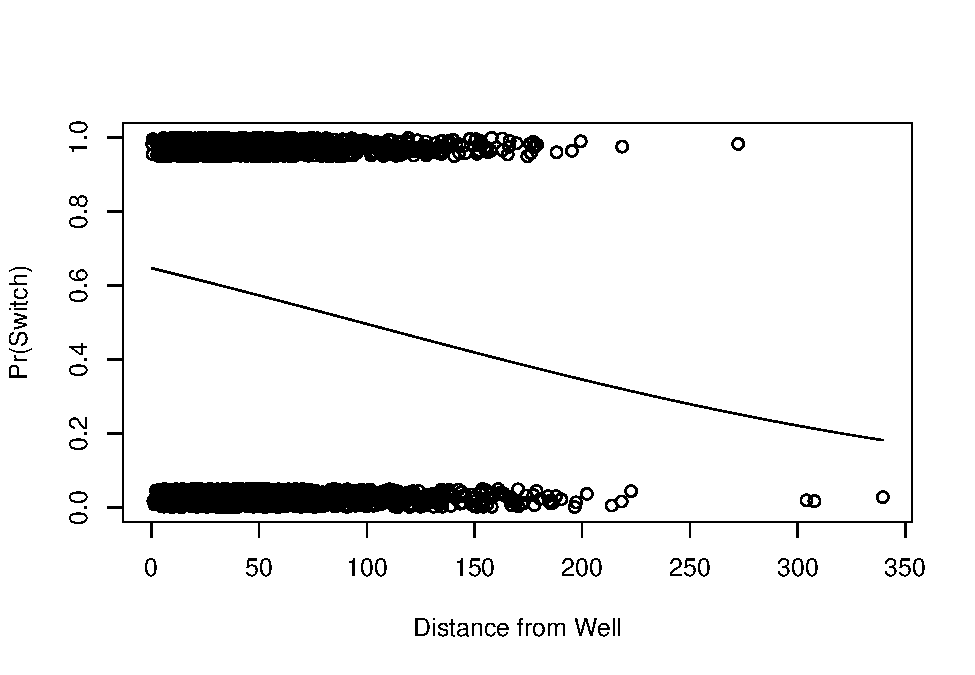
\includegraphics{14.3_files/figure-latex/unnamed-chunk-3-1.pdf}

C:

Make a residual plot and binned residual plot as in Figure 14.8.

\begin{Shaded}
\begin{Highlighting}[]
\CommentTok{\#Residual plot}
\FunctionTok{plot}\NormalTok{(fit\_1}\SpecialCharTok{$}\NormalTok{fitted.values, fit\_1}\SpecialCharTok{$}\NormalTok{residuals, }\AttributeTok{main =} \StringTok{"Residual Plot"}\NormalTok{,}
     \AttributeTok{xlab =} \StringTok{"Estimated Pr(switching)"}\NormalTok{, }\AttributeTok{ylab =} \StringTok{"Residual"}\NormalTok{)}
\end{Highlighting}
\end{Shaded}

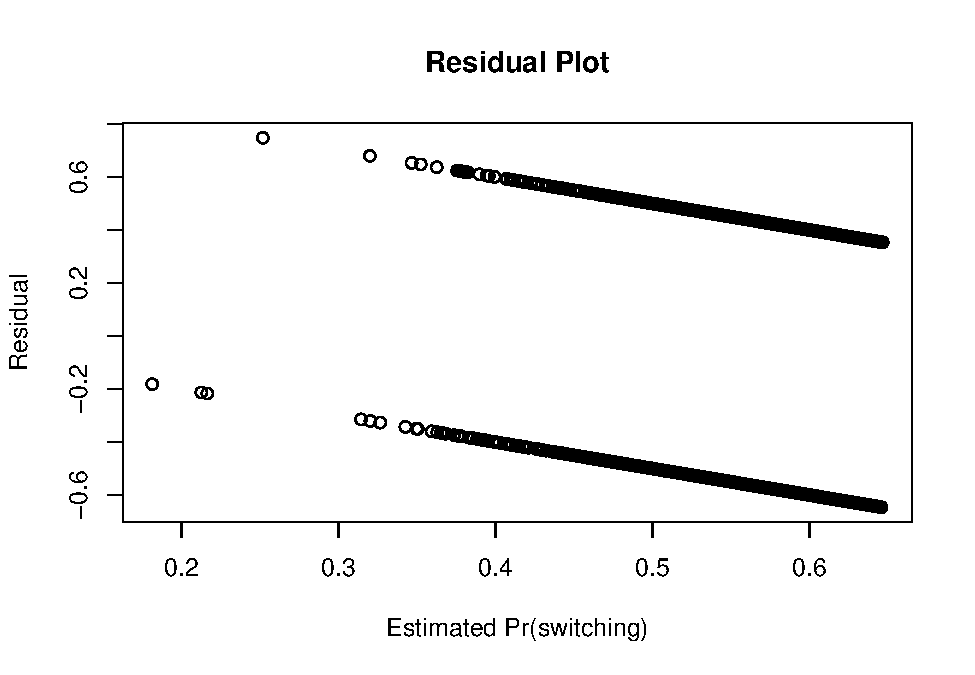
\includegraphics{14.3_files/figure-latex/unnamed-chunk-4-1.pdf}

\begin{Shaded}
\begin{Highlighting}[]
\CommentTok{\#using rstanarm library}
\FunctionTok{pp\_check}\NormalTok{(fit\_1, }\AttributeTok{plotfun =} \StringTok{"error\_binned"}\NormalTok{)}
\end{Highlighting}
\end{Shaded}

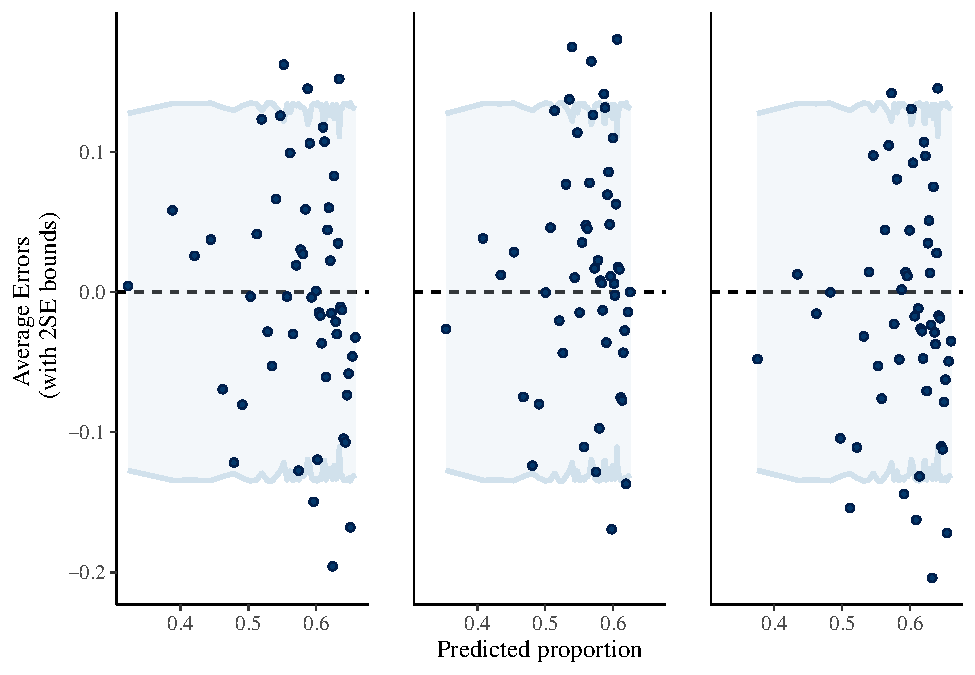
\includegraphics{14.3_files/figure-latex/unnamed-chunk-4-2.pdf}

\begin{Shaded}
\begin{Highlighting}[]
\CommentTok{\#using arm (https://rdrr.io/cran/arm/man/binnedplot.html), more like book graph}
\NormalTok{arm}\SpecialCharTok{::}\FunctionTok{binnedplot}\NormalTok{(}\AttributeTok{x =}\NormalTok{ fit\_1}\SpecialCharTok{$}\NormalTok{fitted.values, fit\_1}\SpecialCharTok{$}\NormalTok{residuals,}
                \AttributeTok{xlab =} \StringTok{"Estimated Pr(Switching)"}\NormalTok{, }
                \AttributeTok{main =} \StringTok{"Binned Residual vs. Predicted Values"}\NormalTok{, }
                \AttributeTok{col.int =} \StringTok{"gray"}\NormalTok{, }\AttributeTok{nclass =} \DecValTok{40}\NormalTok{)}
\end{Highlighting}
\end{Shaded}

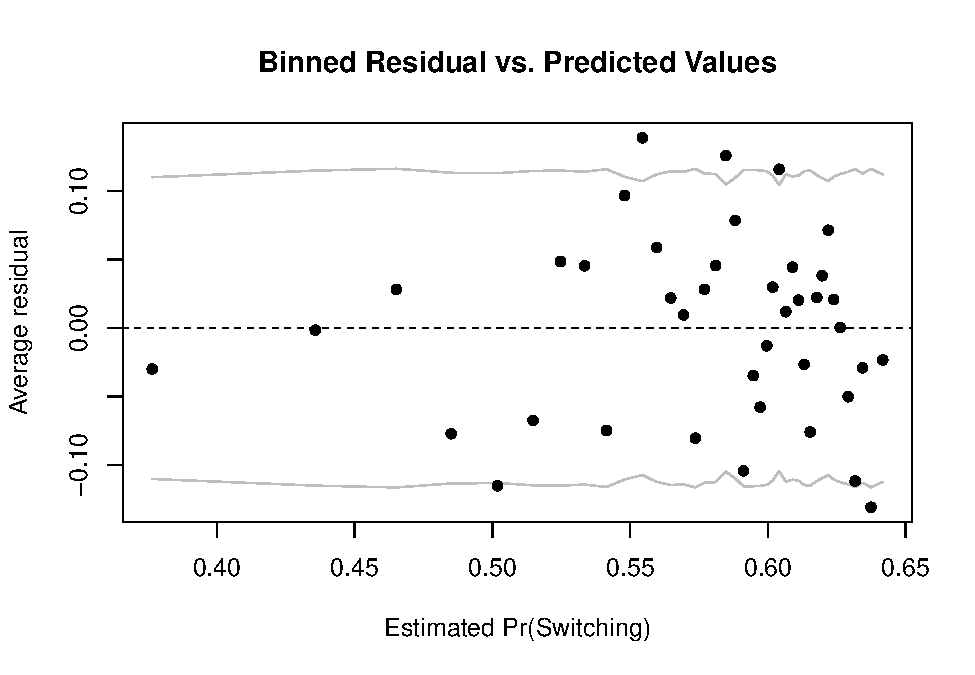
\includegraphics{14.3_files/figure-latex/unnamed-chunk-4-3.pdf}

D:

Compute the error rate of the fitted model and compare to the error rate
of the null model.

\begin{Shaded}
\begin{Highlighting}[]
\CommentTok{\#calculate predictions}
\NormalTok{wells}\SpecialCharTok{$}\NormalTok{predicted }\OtherTok{\textless{}{-}} \FunctionTok{predict}\NormalTok{(fit\_1, }\AttributeTok{newdata =}\NormalTok{ wells, }\AttributeTok{type =} \StringTok{"response"}\NormalTok{)}

\CommentTok{\#fit null model}
\NormalTok{null\_model }\OtherTok{\textless{}{-}} \FunctionTok{stan\_glm}\NormalTok{(}\AttributeTok{formula =} \ControlFlowTok{switch} \SpecialCharTok{\textasciitilde{}} \DecValTok{1}\NormalTok{, }\AttributeTok{family=}\FunctionTok{binomial}\NormalTok{(}\AttributeTok{link=}\StringTok{"logit"}\NormalTok{),}
          \AttributeTok{data=}\NormalTok{wells)}
\end{Highlighting}
\end{Shaded}

\begin{verbatim}
## 
## SAMPLING FOR MODEL 'bernoulli' NOW (CHAIN 1).
## Chain 1: 
## Chain 1: Gradient evaluation took 0.000168 seconds
## Chain 1: 1000 transitions using 10 leapfrog steps per transition would take 1.68 seconds.
## Chain 1: Adjust your expectations accordingly!
## Chain 1: 
## Chain 1: 
## Chain 1: Iteration:    1 / 2000 [  0%]  (Warmup)
## Chain 1: Iteration:  200 / 2000 [ 10%]  (Warmup)
## Chain 1: Iteration:  400 / 2000 [ 20%]  (Warmup)
## Chain 1: Iteration:  600 / 2000 [ 30%]  (Warmup)
## Chain 1: Iteration:  800 / 2000 [ 40%]  (Warmup)
## Chain 1: Iteration: 1000 / 2000 [ 50%]  (Warmup)
## Chain 1: Iteration: 1001 / 2000 [ 50%]  (Sampling)
## Chain 1: Iteration: 1200 / 2000 [ 60%]  (Sampling)
## Chain 1: Iteration: 1400 / 2000 [ 70%]  (Sampling)
## Chain 1: Iteration: 1600 / 2000 [ 80%]  (Sampling)
## Chain 1: Iteration: 1800 / 2000 [ 90%]  (Sampling)
## Chain 1: Iteration: 2000 / 2000 [100%]  (Sampling)
## Chain 1: 
## Chain 1:  Elapsed Time: 0.633203 seconds (Warm-up)
## Chain 1:                0.727796 seconds (Sampling)
## Chain 1:                1.361 seconds (Total)
## Chain 1: 
## 
## SAMPLING FOR MODEL 'bernoulli' NOW (CHAIN 2).
## Chain 2: 
## Chain 2: Gradient evaluation took 0.000148 seconds
## Chain 2: 1000 transitions using 10 leapfrog steps per transition would take 1.48 seconds.
## Chain 2: Adjust your expectations accordingly!
## Chain 2: 
## Chain 2: 
## Chain 2: Iteration:    1 / 2000 [  0%]  (Warmup)
## Chain 2: Iteration:  200 / 2000 [ 10%]  (Warmup)
## Chain 2: Iteration:  400 / 2000 [ 20%]  (Warmup)
## Chain 2: Iteration:  600 / 2000 [ 30%]  (Warmup)
## Chain 2: Iteration:  800 / 2000 [ 40%]  (Warmup)
## Chain 2: Iteration: 1000 / 2000 [ 50%]  (Warmup)
## Chain 2: Iteration: 1001 / 2000 [ 50%]  (Sampling)
## Chain 2: Iteration: 1200 / 2000 [ 60%]  (Sampling)
## Chain 2: Iteration: 1400 / 2000 [ 70%]  (Sampling)
## Chain 2: Iteration: 1600 / 2000 [ 80%]  (Sampling)
## Chain 2: Iteration: 1800 / 2000 [ 90%]  (Sampling)
## Chain 2: Iteration: 2000 / 2000 [100%]  (Sampling)
## Chain 2: 
## Chain 2:  Elapsed Time: 0.683908 seconds (Warm-up)
## Chain 2:                0.783036 seconds (Sampling)
## Chain 2:                1.46694 seconds (Total)
## Chain 2: 
## 
## SAMPLING FOR MODEL 'bernoulli' NOW (CHAIN 3).
## Chain 3: 
## Chain 3: Gradient evaluation took 0.000145 seconds
## Chain 3: 1000 transitions using 10 leapfrog steps per transition would take 1.45 seconds.
## Chain 3: Adjust your expectations accordingly!
## Chain 3: 
## Chain 3: 
## Chain 3: Iteration:    1 / 2000 [  0%]  (Warmup)
## Chain 3: Iteration:  200 / 2000 [ 10%]  (Warmup)
## Chain 3: Iteration:  400 / 2000 [ 20%]  (Warmup)
## Chain 3: Iteration:  600 / 2000 [ 30%]  (Warmup)
## Chain 3: Iteration:  800 / 2000 [ 40%]  (Warmup)
## Chain 3: Iteration: 1000 / 2000 [ 50%]  (Warmup)
## Chain 3: Iteration: 1001 / 2000 [ 50%]  (Sampling)
## Chain 3: Iteration: 1200 / 2000 [ 60%]  (Sampling)
## Chain 3: Iteration: 1400 / 2000 [ 70%]  (Sampling)
## Chain 3: Iteration: 1600 / 2000 [ 80%]  (Sampling)
## Chain 3: Iteration: 1800 / 2000 [ 90%]  (Sampling)
## Chain 3: Iteration: 2000 / 2000 [100%]  (Sampling)
## Chain 3: 
## Chain 3:  Elapsed Time: 0.656143 seconds (Warm-up)
## Chain 3:                0.699383 seconds (Sampling)
## Chain 3:                1.35553 seconds (Total)
## Chain 3: 
## 
## SAMPLING FOR MODEL 'bernoulli' NOW (CHAIN 4).
## Chain 4: 
## Chain 4: Gradient evaluation took 0.000148 seconds
## Chain 4: 1000 transitions using 10 leapfrog steps per transition would take 1.48 seconds.
## Chain 4: Adjust your expectations accordingly!
## Chain 4: 
## Chain 4: 
## Chain 4: Iteration:    1 / 2000 [  0%]  (Warmup)
## Chain 4: Iteration:  200 / 2000 [ 10%]  (Warmup)
## Chain 4: Iteration:  400 / 2000 [ 20%]  (Warmup)
## Chain 4: Iteration:  600 / 2000 [ 30%]  (Warmup)
## Chain 4: Iteration:  800 / 2000 [ 40%]  (Warmup)
## Chain 4: Iteration: 1000 / 2000 [ 50%]  (Warmup)
## Chain 4: Iteration: 1001 / 2000 [ 50%]  (Sampling)
## Chain 4: Iteration: 1200 / 2000 [ 60%]  (Sampling)
## Chain 4: Iteration: 1400 / 2000 [ 70%]  (Sampling)
## Chain 4: Iteration: 1600 / 2000 [ 80%]  (Sampling)
## Chain 4: Iteration: 1800 / 2000 [ 90%]  (Sampling)
## Chain 4: Iteration: 2000 / 2000 [100%]  (Sampling)
## Chain 4: 
## Chain 4:  Elapsed Time: 0.658551 seconds (Warm-up)
## Chain 4:                0.832231 seconds (Sampling)
## Chain 4:                1.49078 seconds (Total)
## Chain 4:
\end{verbatim}

\begin{Shaded}
\begin{Highlighting}[]
\CommentTok{\#code from p 273 to compute error rate of models}
\NormalTok{error\_rate\_fit }\OtherTok{\textless{}{-}} \FunctionTok{mean}\NormalTok{((wells}\SpecialCharTok{$}\NormalTok{predicted}\SpecialCharTok{\textgreater{}}\FloatTok{0.5} \SpecialCharTok{\&}\NormalTok{ wells}\SpecialCharTok{$}\ControlFlowTok{switch}\SpecialCharTok{==}\DecValTok{0}\NormalTok{) }\SpecialCharTok{|}\NormalTok{ (wells}\SpecialCharTok{$}\NormalTok{predicted}\SpecialCharTok{\textless{}}\FloatTok{0.5} \SpecialCharTok{\&}\NormalTok{ wells}\SpecialCharTok{$}\ControlFlowTok{switch}\SpecialCharTok{==}\DecValTok{1}\NormalTok{))}

\CommentTok{\#We can compare it to the error rate of the null model, which is simply to assign the same probability to each yi. This is simply logistic regression with only a constant term, and the estimated probability will simply be the proportion of 1’s in the data, or p = n i=1 yi/n (recalling that each yi = 0 or 1). The error rate of the null model is then p or 1−p, whichever is lower}

\NormalTok{prop\_1\_in\_data }\OtherTok{\textless{}{-}} \FunctionTok{table}\NormalTok{(wells}\SpecialCharTok{$}\ControlFlowTok{switch}\NormalTok{)}

\NormalTok{prop\_1\_in\_data }\OtherTok{\textless{}{-}} \DecValTok{1737}\SpecialCharTok{/}\DecValTok{3020}

\NormalTok{error\_rate\_null }\OtherTok{\textless{}{-}} \DecValTok{1} \SpecialCharTok{{-}}\NormalTok{ prop\_1\_in\_data}

\NormalTok{df }\OtherTok{\textless{}{-}} \FunctionTok{data.frame}\NormalTok{(}
  \StringTok{"model"} \OtherTok{\textless{}{-}} \FunctionTok{c}\NormalTok{(}\StringTok{"Fitted"}\NormalTok{, }\StringTok{"Null"}\NormalTok{),}
  \StringTok{"error"} \OtherTok{\textless{}{-}} \FunctionTok{c}\NormalTok{(error\_rate\_fit, error\_rate\_null))}

\FunctionTok{colnames}\NormalTok{(df) }\OtherTok{\textless{}{-}} \FunctionTok{c}\NormalTok{(}\StringTok{"model"}\NormalTok{, }\StringTok{"error"}\NormalTok{)}

\FunctionTok{print}\NormalTok{(}\FunctionTok{paste}\NormalTok{(}\StringTok{"Fitted model error: "}\NormalTok{, }\FunctionTok{round}\NormalTok{(error\_rate\_fit, }\DecValTok{3}\NormalTok{)))}
\end{Highlighting}
\end{Shaded}

\begin{verbatim}
## [1] "Fitted model error:  0.405"
\end{verbatim}

\begin{Shaded}
\begin{Highlighting}[]
\FunctionTok{print}\NormalTok{(}\FunctionTok{paste}\NormalTok{(}\StringTok{"Null model error: "}\NormalTok{, }\FunctionTok{round}\NormalTok{(error\_rate\_null, }\DecValTok{3}\NormalTok{)))}
\end{Highlighting}
\end{Shaded}

\begin{verbatim}
## [1] "Null model error:  0.425"
\end{verbatim}

\begin{Shaded}
\begin{Highlighting}[]
\NormalTok{bp }\OtherTok{\textless{}{-}} \FunctionTok{barplot}\NormalTok{(df}\SpecialCharTok{$}\NormalTok{error, }\AttributeTok{names.arg =}\NormalTok{ df}\SpecialCharTok{$}\NormalTok{model, }\AttributeTok{main =} \StringTok{"Barplot of Fitted vs Null Model Error"}\NormalTok{)}
\FunctionTok{text}\NormalTok{(bp, }\DecValTok{0}\NormalTok{, }\FunctionTok{round}\NormalTok{(df}\SpecialCharTok{$}\NormalTok{error, }\DecValTok{3}\NormalTok{),}\AttributeTok{cex=}\DecValTok{1}\NormalTok{,}\AttributeTok{pos=}\DecValTok{3}\NormalTok{) }
\end{Highlighting}
\end{Shaded}

\includegraphics{14.3_files/figure-latex/unnamed-chunk-5-1.pdf}

E:

Create indicator variables corresponding to dist \textless{} 100; dist
between 100 and 200; and dist \textgreater{} 200. Fit a logistic
regression for Pr(switch) using these indicators. With this new model,
repeat the computations and graphs for part (a) of this exercise.

Create indicator variables and fit model:

\begin{Shaded}
\begin{Highlighting}[]
\NormalTok{wells}\SpecialCharTok{$}\NormalTok{less\_100 }\OtherTok{\textless{}{-}} \FunctionTok{ifelse}\NormalTok{(wells}\SpecialCharTok{$}\NormalTok{dist }\SpecialCharTok{\textless{}} \DecValTok{100}\NormalTok{, }\DecValTok{1}\NormalTok{, }\DecValTok{0}\NormalTok{)}
\NormalTok{wells}\SpecialCharTok{$}\NormalTok{greater\_200 }\OtherTok{\textless{}{-}} \FunctionTok{ifelse}\NormalTok{(wells}\SpecialCharTok{$}\NormalTok{dist }\SpecialCharTok{\textgreater{}} \DecValTok{200}\NormalTok{, }\DecValTok{1}\NormalTok{, }\DecValTok{0}\NormalTok{)}
\NormalTok{wells}\SpecialCharTok{$}\NormalTok{between }\OtherTok{\textless{}{-}} \FunctionTok{ifelse}\NormalTok{(wells}\SpecialCharTok{$}\NormalTok{dist }\SpecialCharTok{\textless{}} \DecValTok{200} \SpecialCharTok{\&}\NormalTok{ wells}\SpecialCharTok{$}\NormalTok{dist }\SpecialCharTok{\textgreater{}} \DecValTok{100}\NormalTok{, }\DecValTok{1}\NormalTok{, }\DecValTok{0}\NormalTok{)}

\NormalTok{wells}\SpecialCharTok{$}\NormalTok{less\_100 }\OtherTok{\textless{}{-}} \FunctionTok{as.factor}\NormalTok{(wells}\SpecialCharTok{$}\NormalTok{less\_100)}
\NormalTok{wells}\SpecialCharTok{$}\NormalTok{greater\_200 }\OtherTok{\textless{}{-}} \FunctionTok{as.factor}\NormalTok{(wells}\SpecialCharTok{$}\NormalTok{greater\_200)}
\NormalTok{wells}\SpecialCharTok{$}\NormalTok{between }\OtherTok{\textless{}{-}} \FunctionTok{as.factor}\NormalTok{(wells}\SpecialCharTok{$}\NormalTok{between)}

\NormalTok{fit\_2 }\OtherTok{\textless{}{-}} \FunctionTok{stan\_glm}\NormalTok{(}\AttributeTok{formula =} \ControlFlowTok{switch} \SpecialCharTok{\textasciitilde{}}\NormalTok{ less\_100 }\SpecialCharTok{+}\NormalTok{ greater\_200 }\SpecialCharTok{+}\NormalTok{ between, }\AttributeTok{family=}\FunctionTok{binomial}\NormalTok{(}\AttributeTok{link=}\StringTok{"logit"}\NormalTok{),}
          \AttributeTok{data=}\NormalTok{wells)}
\end{Highlighting}
\end{Shaded}

\begin{verbatim}
## 
## SAMPLING FOR MODEL 'bernoulli' NOW (CHAIN 1).
## Chain 1: 
## Chain 1: Gradient evaluation took 5.6e-05 seconds
## Chain 1: 1000 transitions using 10 leapfrog steps per transition would take 0.56 seconds.
## Chain 1: Adjust your expectations accordingly!
## Chain 1: 
## Chain 1: 
## Chain 1: Iteration:    1 / 2000 [  0%]  (Warmup)
## Chain 1: Iteration:  200 / 2000 [ 10%]  (Warmup)
## Chain 1: Iteration:  400 / 2000 [ 20%]  (Warmup)
## Chain 1: Iteration:  600 / 2000 [ 30%]  (Warmup)
## Chain 1: Iteration:  800 / 2000 [ 40%]  (Warmup)
## Chain 1: Iteration: 1000 / 2000 [ 50%]  (Warmup)
## Chain 1: Iteration: 1001 / 2000 [ 50%]  (Sampling)
## Chain 1: Iteration: 1200 / 2000 [ 60%]  (Sampling)
## Chain 1: Iteration: 1400 / 2000 [ 70%]  (Sampling)
## Chain 1: Iteration: 1600 / 2000 [ 80%]  (Sampling)
## Chain 1: Iteration: 1800 / 2000 [ 90%]  (Sampling)
## Chain 1: Iteration: 2000 / 2000 [100%]  (Sampling)
## Chain 1: 
## Chain 1:  Elapsed Time: 6.65626 seconds (Warm-up)
## Chain 1:                7.69363 seconds (Sampling)
## Chain 1:                14.3499 seconds (Total)
## Chain 1: 
## 
## SAMPLING FOR MODEL 'bernoulli' NOW (CHAIN 2).
## Chain 2: 
## Chain 2: Gradient evaluation took 4.5e-05 seconds
## Chain 2: 1000 transitions using 10 leapfrog steps per transition would take 0.45 seconds.
## Chain 2: Adjust your expectations accordingly!
## Chain 2: 
## Chain 2: 
## Chain 2: Iteration:    1 / 2000 [  0%]  (Warmup)
## Chain 2: Iteration:  200 / 2000 [ 10%]  (Warmup)
## Chain 2: Iteration:  400 / 2000 [ 20%]  (Warmup)
## Chain 2: Iteration:  600 / 2000 [ 30%]  (Warmup)
## Chain 2: Iteration:  800 / 2000 [ 40%]  (Warmup)
## Chain 2: Iteration: 1000 / 2000 [ 50%]  (Warmup)
## Chain 2: Iteration: 1001 / 2000 [ 50%]  (Sampling)
## Chain 2: Iteration: 1200 / 2000 [ 60%]  (Sampling)
## Chain 2: Iteration: 1400 / 2000 [ 70%]  (Sampling)
## Chain 2: Iteration: 1600 / 2000 [ 80%]  (Sampling)
## Chain 2: Iteration: 1800 / 2000 [ 90%]  (Sampling)
## Chain 2: Iteration: 2000 / 2000 [100%]  (Sampling)
## Chain 2: 
## Chain 2:  Elapsed Time: 6.66636 seconds (Warm-up)
## Chain 2:                6.53439 seconds (Sampling)
## Chain 2:                13.2008 seconds (Total)
## Chain 2: 
## 
## SAMPLING FOR MODEL 'bernoulli' NOW (CHAIN 3).
## Chain 3: 
## Chain 3: Gradient evaluation took 4.6e-05 seconds
## Chain 3: 1000 transitions using 10 leapfrog steps per transition would take 0.46 seconds.
## Chain 3: Adjust your expectations accordingly!
## Chain 3: 
## Chain 3: 
## Chain 3: Iteration:    1 / 2000 [  0%]  (Warmup)
## Chain 3: Iteration:  200 / 2000 [ 10%]  (Warmup)
## Chain 3: Iteration:  400 / 2000 [ 20%]  (Warmup)
## Chain 3: Iteration:  600 / 2000 [ 30%]  (Warmup)
## Chain 3: Iteration:  800 / 2000 [ 40%]  (Warmup)
## Chain 3: Iteration: 1000 / 2000 [ 50%]  (Warmup)
## Chain 3: Iteration: 1001 / 2000 [ 50%]  (Sampling)
## Chain 3: Iteration: 1200 / 2000 [ 60%]  (Sampling)
## Chain 3: Iteration: 1400 / 2000 [ 70%]  (Sampling)
## Chain 3: Iteration: 1600 / 2000 [ 80%]  (Sampling)
## Chain 3: Iteration: 1800 / 2000 [ 90%]  (Sampling)
## Chain 3: Iteration: 2000 / 2000 [100%]  (Sampling)
## Chain 3: 
## Chain 3:  Elapsed Time: 6.82362 seconds (Warm-up)
## Chain 3:                7.38623 seconds (Sampling)
## Chain 3:                14.2098 seconds (Total)
## Chain 3: 
## 
## SAMPLING FOR MODEL 'bernoulli' NOW (CHAIN 4).
## Chain 4: 
## Chain 4: Gradient evaluation took 5e-05 seconds
## Chain 4: 1000 transitions using 10 leapfrog steps per transition would take 0.5 seconds.
## Chain 4: Adjust your expectations accordingly!
## Chain 4: 
## Chain 4: 
## Chain 4: Iteration:    1 / 2000 [  0%]  (Warmup)
## Chain 4: Iteration:  200 / 2000 [ 10%]  (Warmup)
## Chain 4: Iteration:  400 / 2000 [ 20%]  (Warmup)
## Chain 4: Iteration:  600 / 2000 [ 30%]  (Warmup)
## Chain 4: Iteration:  800 / 2000 [ 40%]  (Warmup)
## Chain 4: Iteration: 1000 / 2000 [ 50%]  (Warmup)
## Chain 4: Iteration: 1001 / 2000 [ 50%]  (Sampling)
## Chain 4: Iteration: 1200 / 2000 [ 60%]  (Sampling)
## Chain 4: Iteration: 1400 / 2000 [ 70%]  (Sampling)
## Chain 4: Iteration: 1600 / 2000 [ 80%]  (Sampling)
## Chain 4: Iteration: 1800 / 2000 [ 90%]  (Sampling)
## Chain 4: Iteration: 2000 / 2000 [100%]  (Sampling)
## Chain 4: 
## Chain 4:  Elapsed Time: 7.03871 seconds (Warm-up)
## Chain 4:                7.69407 seconds (Sampling)
## Chain 4:                14.7328 seconds (Total)
## Chain 4:
\end{verbatim}

Distance from well vs Pr(switch):

\begin{Shaded}
\begin{Highlighting}[]
\CommentTok{\#code from p 252 in text}
\NormalTok{jitter\_binary }\OtherTok{\textless{}{-}} \ControlFlowTok{function}\NormalTok{(a, }\AttributeTok{jitt=}\FloatTok{0.05}\NormalTok{)\{}
\FunctionTok{ifelse}\NormalTok{(a}\SpecialCharTok{==}\DecValTok{0}\NormalTok{, }\FunctionTok{runif}\NormalTok{(}\FunctionTok{length}\NormalTok{(a), }\DecValTok{0}\NormalTok{, jitt), }\FunctionTok{runif}\NormalTok{(}\FunctionTok{length}\NormalTok{(a), }\DecValTok{1} \SpecialCharTok{{-}}\NormalTok{ jitt, }\DecValTok{1}\NormalTok{))}
\NormalTok{\}}

\NormalTok{wells}\SpecialCharTok{$}\NormalTok{switch\_jitter }\OtherTok{\textless{}{-}} \FunctionTok{jitter\_binary}\NormalTok{(wells}\SpecialCharTok{$}\ControlFlowTok{switch}\NormalTok{)}
\FunctionTok{plot}\NormalTok{(wells}\SpecialCharTok{$}\NormalTok{dist, wells}\SpecialCharTok{$}\NormalTok{switch\_jitter, }\AttributeTok{xlab =} \StringTok{"Distance from Well"}\NormalTok{, }\AttributeTok{ylab =} \StringTok{"Pr(Switch)"}\NormalTok{)}
\FunctionTok{curve}\NormalTok{(}\FunctionTok{invlogit}\NormalTok{(}\FunctionTok{coef}\NormalTok{(fit\_2)[}\DecValTok{1}\NormalTok{] }\SpecialCharTok{+} \FunctionTok{coef}\NormalTok{(fit\_2)[}\DecValTok{2}\NormalTok{]}\SpecialCharTok{*}\NormalTok{x), }\AttributeTok{add=}\ConstantTok{TRUE}\NormalTok{)}
\end{Highlighting}
\end{Shaded}

\includegraphics{14.3_files/figure-latex/unnamed-chunk-7-1.pdf}

Residual and Binned Plots:

\begin{Shaded}
\begin{Highlighting}[]
\CommentTok{\#Residual plot}
\FunctionTok{plot}\NormalTok{(fit\_2}\SpecialCharTok{$}\NormalTok{fitted.values, fit\_2}\SpecialCharTok{$}\NormalTok{residuals, }\AttributeTok{main =} \StringTok{"Residual Plot"}\NormalTok{,}
     \AttributeTok{xlab =} \StringTok{"Estimated Pr(switching)"}\NormalTok{, }\AttributeTok{ylab =} \StringTok{"Residual"}\NormalTok{)}
\end{Highlighting}
\end{Shaded}

\includegraphics{14.3_files/figure-latex/unnamed-chunk-8-1.pdf}

\begin{Shaded}
\begin{Highlighting}[]
\CommentTok{\#using rstanarm library}
\FunctionTok{pp\_check}\NormalTok{(fit\_2, }\AttributeTok{plotfun =} \StringTok{"error\_binned"}\NormalTok{)}
\end{Highlighting}
\end{Shaded}

\includegraphics{14.3_files/figure-latex/unnamed-chunk-8-2.pdf}

\begin{Shaded}
\begin{Highlighting}[]
\CommentTok{\#using arm (https://rdrr.io/cran/arm/man/binnedplot.html), more like book graph}
\NormalTok{arm}\SpecialCharTok{::}\FunctionTok{binnedplot}\NormalTok{(}\AttributeTok{x =}\NormalTok{ fit\_2}\SpecialCharTok{$}\NormalTok{fitted.values, fit\_2}\SpecialCharTok{$}\NormalTok{residuals,}
                \AttributeTok{xlab =} \StringTok{"Estimated Pr(Switching)"}\NormalTok{, }
                \AttributeTok{main =} \StringTok{"Binned Residual vs. Predicted Values"}\NormalTok{, }
                \AttributeTok{col.int =} \StringTok{"gray"}\NormalTok{, }\AttributeTok{nclass =} \DecValTok{40}\NormalTok{)}
\end{Highlighting}
\end{Shaded}

\includegraphics{14.3_files/figure-latex/unnamed-chunk-8-3.pdf}

Error rate calculation:

\begin{Shaded}
\begin{Highlighting}[]
\CommentTok{\#calculate predictions}
\NormalTok{wells}\SpecialCharTok{$}\NormalTok{predicted\_2 }\OtherTok{\textless{}{-}} \FunctionTok{predict}\NormalTok{(fit\_2, }\AttributeTok{newdata =}\NormalTok{ wells, }\AttributeTok{type =} \StringTok{"response"}\NormalTok{)}


\CommentTok{\#code from p 273 to compute error rate of models}
\NormalTok{error\_rate\_fit\_2 }\OtherTok{\textless{}{-}} \FunctionTok{mean}\NormalTok{((wells}\SpecialCharTok{$}\NormalTok{predicted\_2}\SpecialCharTok{\textgreater{}}\FloatTok{0.5} \SpecialCharTok{\&}\NormalTok{ wells}\SpecialCharTok{$}\ControlFlowTok{switch}\SpecialCharTok{==}\DecValTok{0}\NormalTok{) }\SpecialCharTok{|}\NormalTok{ (wells}\SpecialCharTok{$}\NormalTok{predicted\_2}\SpecialCharTok{\textless{}}\FloatTok{0.5} \SpecialCharTok{\&}\NormalTok{ wells}\SpecialCharTok{$}\ControlFlowTok{switch}\SpecialCharTok{==}\DecValTok{1}\NormalTok{))}

\CommentTok{\#We can compare it to the error rate of the null model, which is simply to assign the same probability to each yi. This is simply logistic regression with only a constant term, and the estimated probability will simply be the proportion of 1’s in the data, or p = n i=1 yi/n (recalling that each yi = 0 or 1). The error rate of the null model is then p or 1−p, whichever is lower}

\NormalTok{prop\_1\_in\_data }\OtherTok{\textless{}{-}} \FunctionTok{table}\NormalTok{(wells}\SpecialCharTok{$}\ControlFlowTok{switch}\NormalTok{)}

\NormalTok{prop\_1\_in\_data }\OtherTok{\textless{}{-}} \DecValTok{1737}\SpecialCharTok{/}\DecValTok{3020}

\NormalTok{error\_rate\_null }\OtherTok{\textless{}{-}} \DecValTok{1} \SpecialCharTok{{-}}\NormalTok{ prop\_1\_in\_data}

\NormalTok{df2 }\OtherTok{\textless{}{-}} \FunctionTok{data.frame}\NormalTok{(}
  \StringTok{"model"} \OtherTok{\textless{}{-}} \FunctionTok{c}\NormalTok{(}\StringTok{"Fitted"}\NormalTok{, }\StringTok{"Null"}\NormalTok{),}
  \StringTok{"error"} \OtherTok{\textless{}{-}} \FunctionTok{c}\NormalTok{(error\_rate\_fit\_2, error\_rate\_null))}

\FunctionTok{colnames}\NormalTok{(df2) }\OtherTok{\textless{}{-}} \FunctionTok{c}\NormalTok{(}\StringTok{"model"}\NormalTok{, }\StringTok{"error"}\NormalTok{)}

\FunctionTok{print}\NormalTok{(}\FunctionTok{paste}\NormalTok{(}\StringTok{"Fitted model error: "}\NormalTok{, }\FunctionTok{round}\NormalTok{(error\_rate\_fit\_2, }\DecValTok{3}\NormalTok{)))}
\end{Highlighting}
\end{Shaded}

\begin{verbatim}
## [1] "Fitted model error:  0.409"
\end{verbatim}

\begin{Shaded}
\begin{Highlighting}[]
\FunctionTok{print}\NormalTok{(}\FunctionTok{paste}\NormalTok{(}\StringTok{"Null model error: "}\NormalTok{, }\FunctionTok{round}\NormalTok{(error\_rate\_null, }\DecValTok{3}\NormalTok{)))}
\end{Highlighting}
\end{Shaded}

\begin{verbatim}
## [1] "Null model error:  0.425"
\end{verbatim}

\begin{Shaded}
\begin{Highlighting}[]
\NormalTok{bp }\OtherTok{\textless{}{-}} \FunctionTok{barplot}\NormalTok{(df}\SpecialCharTok{$}\NormalTok{error, }\AttributeTok{names.arg =}\NormalTok{ df2}\SpecialCharTok{$}\NormalTok{model, }\AttributeTok{main =} \StringTok{"Barplot of Fitted vs Null Model Error"}\NormalTok{)}
\FunctionTok{text}\NormalTok{(bp, }\DecValTok{0}\NormalTok{, }\FunctionTok{round}\NormalTok{(df2}\SpecialCharTok{$}\NormalTok{error, }\DecValTok{3}\NormalTok{),}\AttributeTok{cex=}\DecValTok{1}\NormalTok{,}\AttributeTok{pos=}\DecValTok{3}\NormalTok{) }
\end{Highlighting}
\end{Shaded}

\includegraphics{14.3_files/figure-latex/unnamed-chunk-9-1.pdf}

This model had an error rate of 0.4092715, which is slightly higher
compared to our original model's error rate of 0.4056291. Thus, in terms
of making predictions on this dataset, our original model is better than
using this indicator model.

\end{document}
